\documentclass[prb,aps,amssym,nofootinbib,floatfix,notitlepage]{revtex4-1} 
\usepackage{graphicx,natbib}
\usepackage{amsmath}
\usepackage{amsfonts}
\usepackage{siunitx}
\usepackage{bbm}
\usepackage[bookmarks=true,pdfcreator={Adrian Del Maestro}]{hyperref}
\usepackage{url}

\renewcommand{\vec}[1]{\boldsymbol{#1}}
\newcommand{\e}[1]{\mathrm{e}^{#1}}
\newcommand{\sgn}[1]{\mathrm{sgn}(#1)}
\renewcommand{\eqref}[1]{Eq.~(\ref{#1})}
\newcommand{\R}{\vec{R}}
\newcommand{\T}{\mathcal{T}}

\begin{document}
\title{Path Integral Monte Carlo and the Worm Algorithm in the Spatial
Continuum}
\author{Adrian Del Maestro}
\email{Adrian.DelMaestro@uvm.edu}
\affiliation{Department of Physics, University of Vermont, Burlington, VT 05405, USA}

\date{\today}
\maketitle

The goal of these lecture notes will be to describe a stochastically exact
quantum Monte Carlo method for computing the expectation value of observables
for systems of interacting particles in the spatial continuum described by a
Hamiltonian  which conserves particle number.  The latest
version of the notes can always be found online at
\url{https://github.com/agdelma/pimc-notes} while instructions on how to
obtain, install and run our groups continuous space worm algorithm code are located at
\url{http://code.delmaestro.org}.

\section{Expectation Values and the Partition Function}
%======================================================

We begin with the general definition for the expectation value of some operator
$\hat{\mathcal{O}}$ in terms of a trace over configurations
%
\begin{equation}
    \langle \mathcal{O} \rangle = \frac{1}{\mathcal{Z}} \mathrm{Tr}\, 
    \hat{\mathcal{O}}\e{-\beta \hat{\mathcal{H}}} 
\label{eq:operatorExpectationValue}
\end{equation}
%
where $\beta = 1/k_{\mathrm{B}}T$ with $k_{\mathrm{B}}$ the Boltzmann constant
and the partition function $\mathcal{Z}$ is given by
%
\begin{equation}
    \mathcal{Z} = \mathrm{Tr}\,\e{-\beta \hat{\mathcal{H}}} 
    = \mathrm{Tr}\,\hat{\rho} 
\label{eq:partitionFunction} 
\end{equation}
%
where 
%
\begin{equation}
\hat{\rho} \equiv \e{-\beta \hat{\mathcal{H}}} 
\end{equation}
%
is the density matrix.  In order to compute the trace in
\eqref{eq:partitionFunction} for a given system described by Hamiltonian
$\hat{\mathcal{H}}$ we need to identify a set of convenient basis states
$|\gamma\rangle$ that can be efficiently sampled allowing us to write the
partition function as the direct sum 
%
\begin{align}
    \mathcal{Z} &=  \sum_{\gamma}\langle \gamma | \e{-\beta \hat{\mathcal{H}}}
    |\gamma \rangle \nonumber \\
    &\approx \sum_{\gamma} W(\gamma)
\end{align}
%
where $W(\gamma)$ is a positive real weight corresponding to configuration
state $|\gamma\rangle$.  In the next section we will introduce the specific
form of $|\gamma\rangle$ in terms of the spatial positions of interacting
particles and describe a method for computing the partition function as a sum
of weights.

\section{Path Integral Monte Carlo}
%==================================

The path-integral Monte Carlo method was first introduced by David Ceperley, and a
comprehensive review can be found in Ref.~[\onlinecite{Ceperley:1995gr}]. Here
we will attempt to provide an introduction to the method with sufficient
details to allow for the creation of a simple code.

We are interested in a system of interacting particles described by the
general many-body Hamiltonian:
%
\begin{align}
    \hat{\mathcal{H}} &= \hat{\mathcal{T}} + \hat{\mathcal{V}} \nonumber \\
                      &= -\sum_i^N \frac{\hbar^2}{2m_i} \hat{\vec{\nabla}}_i^2 
    + \sum_{i=1}^N \hat{V}_{i} + \sum_{i < j} \hat{U}_{ij}.
\label{eq:Hamiltonian}
\end{align}
%
It will be convenient to work in first quantized notation, where the $N$
particles in the $d$-dimensional spatial continuum are located at positions
$\vec{r}_i$ with $i=1\ldots N$.  The first term in \eqref{eq:Hamiltonian}
corresponds to the kinetic energy $\hat{\mathcal{T}}$ where $m_i$ is the mass
of the $i^{\text{th}}$ particle. The external potential energy $V(\vec{r_i})$
only depends on the position of a single particle, while the two-body
interaction potential $U(\vec{r}_i-\vec{r}_j)$ is in general a function of the
vector displacement between them.  We will most often work with spherically
symmetric interaction potentials such that $U(\vec{r}_i - \vec{r}_j) =
U(|\vec{r}_i-\vec{r}_j|)$ and we will neglect all self-interactions:
$\hat{U}_{ii} = 0$. A physical system of interest could include trapped
ultra-cold atoms, where $V(\vec{r}_i) \sim |\vec{r}_i|^2$ is a harmonic
trapping potential and the particles interact via an induced dipole-dipole
interaction $U(\vec{r}_i - \vec{r}_j) \sim |\vec{r}_i-\vec{r}_j|^{-3}$.

The most natural basis states $|\gamma\rangle$ in this case are just a
collection of the spatial locations of the $N$ particles, where in the case of
identical particles, the labels are fictitious. We will employ the convenient
short-hand notation 
%
\begin{equation}
    |\R\rangle \equiv |\vec{r}_1, \cdots, \vec{r}_N \rangle
\end{equation}
%
where particle conservation enforces the normalization constraint
%
\begin{equation}
\int \mathcal{D}\R\, |\R\rangle \langle \R | = \mathbbm{1}
\label{eq:Norm}
\end{equation}
%
with 
%
\begin{equation}
    \int\mathcal{D} \R  \equiv \prod_{i=1}^N \int d \vec{r}_i.
\end{equation}
%
In the first-quantized spatial position basis, the partition function can be
written as a $N \times d$ dimensional integral
%
\begin{align}
    \mathcal{Z} &= \mathrm{Tr}\, \e{-\beta \hat{\mathcal{H}}}  \nonumber \\
                &= \int d\vec{r}_1 \cdots \int d\vec{r}_N \langle \vec{r}_1,
    \cdots, \vec{r}_N | \e{-\beta \hat{\mathcal{H}}}| \vec{r}_1, \cdots,
    \vec{r}_N \rangle \nonumber \\
&\equiv \int \mathcal{D} \R \langle \R | \e{-\beta \hat{\mathcal{H}}} | \R
    \rangle.
\label{eq:ZDR}
\end{align}
%
As terms like this will appear quite frequently, it will be useful to define
the elements of the density matrix at inverse temperature $\beta$ in the
spatial basis
%
\begin{equation}
    \rho(\R, \R'; \beta) \equiv \langle \R | \e{-\beta \hat{\mathcal{H}}} |
    \R'\rangle
\end{equation}
%
where all matrix elements are real and positive. We note that in the spatial
continuum, the Hilbert space is uncountably infinite, as the particles can take
on any position in $\mathbbm{R}^d$. This is an important observation that will
guide the strategy we choose in the duration of these notes. Using the
expression for $\rho(\R,\R';\beta)$ we can write the partition function:
%
\begin{equation}
\mathcal{Z} = \int \mathcal{D}\R \, \rho(\R,\R;\beta).
\label{eq:Zrho}
\end{equation}
%

As we have defined the potential operator $\hat{\mathcal{V}}$ to be diagonal in
the position basis, it would be extremely convenient if we could decompose the
density matrix into a product of terms containing $\hat{\mathcal{T}}$ and
$\hat{\mathcal{V}}$.  However, we know that
$[\hat{\mathcal{T}},\hat{\mathcal{V}}] \ne 0$ and thus
%
\begin{align}
    \hat{\rho} &= \e{-\beta(\hat{\mathcal{T}} + \hat{\mathcal{V}})} \nonumber
    \\
&\ne \e{-\beta\hat{\mathcal{T}}}\e{-\beta\hat{\mathcal{V}}}.
\end{align}
%
In fact, by employing the Baker-Campbell-Hausdorff formula we know:
%
\begin{equation}
    \e{\hat{A}+\hat{B}} = \e{\hat{A}}\e{\hat{B}}\e{-\frac{1}{2}[\hat{A},\hat{B}]}
    \label{eq:BCH}
\end{equation}
%
and thus 
%
\begin{equation}
    \hat{\rho} = \e{-\beta\hat{\mathcal{T}}}\e{-\beta\hat{\mathcal{V}}} +
    \mathrm{O}\left(\beta^2\right).
\end{equation}
%
with the error diverging in the interesting (and quantum) low temperature limit
$\beta \gg 1$.  However, we may make the rather self-evident observation that
the Hamiltonian must commute with itself,
$[\hat{\mathcal{H}},\hat{\mathcal{H}}] = 0$ thus
%
\begin{align}
    \hat{\rho} &= \e{-\beta \hat{\mathcal{H}}} \nonumber \\
               &= \e{-\frac{\beta}{2}\hat{\mathcal{H}}
-\frac{\beta}{2}\hat{\mathcal{H}}} \nonumber \\
&= \e{-\frac{\beta}{2}\hat{\mathcal{H}}}\e{-\frac{\beta}{2}\hat{\mathcal{H}}}.
\label{eq:HamCommute}
\end{align}
%
In the position basis, this corresponds to the elements of the density matrix
satisfying a convolution relation
%
\begin{align}
    \rho(\R,\R';\beta) &=  \langle \R | \e{-\beta \hat{\mathcal{H}}} | \R'\rangle \nonumber \\
    &=  \langle \R | \e{-\frac{\beta}{2} \hat{\mathcal{H}}} 
    \e{-\frac{\beta}{2} \hat{\mathcal{H}}}| \R'\rangle \nonumber \\
    &= \int \mathcal{D}\R''\,
    \langle \R | \e{-\frac{\beta}{2} \hat{\mathcal{H}}} | \R''\rangle 
    \langle \R'' | \e{-\frac{\beta}{2} \hat{\mathcal{H}}} | \R'\rangle \nonumber \\
    &= \int \mathcal{D}\R''\,
    \rho\left(\R,\R'';\frac{\beta}{2}\right)
    \rho\left(\R'',\R';\frac{\beta}{2}\right)
\label{eq:rhoConvolution}
\end{align}
%
where have employed the normalization condition in \eqref{eq:Norm} and
we note that the individual density matrices are at a higher effective
temperature: $\beta \to \beta/2 \Rightarrow T \to 2 T$. Now, returning to
\eqref{eq:Zrho}, we can employ this convolution relation $M$ times where $M \in
\mathbbm{Z} \gg 1$ to yield a new expression for the partition function
%
\begin{align}
    \mathcal{Z}  &= \int \mathcal{D}\R\, \rho(\R,\R;\beta) \nonumber \\
                 &= \int \mathcal{D}\R_0 \cdots \int \mathcal{D}\R_{M-1}\,
    \rho\left(\R_0,\R_{1};\frac{\beta}{M}\right) \cdots
    \rho\left(\R_{M-1},\R_{0};\frac{\beta}{M}\right)
    \label{eq:Zconvolution}
\end{align}
%
where we have introduced the new notation
%
\begin{equation}
    |\R_\alpha\rangle \equiv |\vec{r}_{1,\alpha}, \cdots, \vec{r}_{N,\alpha}
    \rangle.
\end{equation}
%
Until now, we have not specified the symmetry of the particles, but for the
duration of these notes we will consider systems of identical bosons and thus
we can write \eqref{eq:Zconvolution} in a more compact form:
%
\begin{align}
    \mathcal{Z}  &= \frac{1}{N!}\sum_{\mathcal{P}} 
    \prod_{\alpha=0}^{M-1}\int \mathcal{D}\R_\alpha\,
    \rho\left(\R_\alpha,\R_{\alpha+1};\frac{\beta}{M}\right)
    \label{eq:Zpermute}
\end{align}
%
where the sum is over all permutations $\mathcal{P}$ of the fictitious particle
labels $i$, and we require
%
\begin{equation}
    |\R_M\rangle = \hat{\mathcal{P}} |\R_0\rangle =
    \left|\vec{r}_{\mathcal{P}(1),0}, \cdots \vec{r}_{\mathcal{P}(N),0} \right \rangle
\end{equation}
%
to ensure the trace is non-zero.

Upon closer examination of the individual terms in the product, we may notice:
%
\begin{equation}
    \langle \R_\alpha | \e{-\frac{\beta}{2}\hat{\mathcal{H}}} | \R_{\alpha+1}
    \rangle = 
    \left \langle \R_\alpha \left | \hat{\mathcal{U}}\left(-i \hbar
    \frac{\beta}{M}\right) \right | \R_{\alpha+1}
    \right \rangle 
\end{equation}
%
where 
%
\begin{equation}
    \hat{\mathcal{U}}(t) \equiv \e{-{i t} \hat{\mathcal{H}}/\hbar}
\end{equation}
%
is the unitary time evolution operator of single particle quantum mechanics.
Through the definition:
%
\begin{equation}
t = - i \hbar \tau
\end{equation}
%
where 
%
\begin{equation}
    \tau \equiv \frac{\beta}{M}
\end{equation}
%
we may identify \eqref{eq:Zpermute} as the partition function of a $N$
particle system which evolves in an \emph{imaginary time} direction. The
configurations of our system now correspond to $M$ discrete classical configurations
corresponding to the positions of the $N$ particles:
$|\vec{r}_{1,\alpha},\cdots,\vec{r}_{N,\alpha}\rangle$ where adjacent configurations
in imaginary time at $\alpha \tau$ and $(\alpha+1)\tau$ are connected via an
insertion of the short-imaginary-time propagator 
\begin{align*}
    \rho(\R_\alpha,\R_{\alpha+1};\tau) 
    &= \langle \R_\alpha| \e{-\frac{\beta}{2}\hat{\mathcal{H}}} | \R_{\alpha+1} \rangle 
     \\ 
     &= \langle \R_\alpha| \hat{\mathcal{U}}(-i \hbar \tau) | \R_{\alpha+1} \rangle.
\end{align*}
This is simply a re-statement of the discrete Feynman path integral
formulation of quantum statistical mechanics \cite{feynman1965quantum}, or
equivalently the quantum-classical mapping, which says that a $d$-dimensional
quantum system can be represented as a $(d+1)$-dimensional classical system,
where the extra $(+1)^{th}$ dimension is potentially subject to an additional
boundary condition.

\subsection{Configurations}
%--------------------------
\label{sec:configurations}

We are now ready to unambiguously identify the configurations that will be
sampled in our Monte Carlo. For a system of $N$ particles, they will consist of
$N$ discrete \emph{worldlines} as shown in Figure~\ref{fig:config}. 
%
% ---------------------------------------------------------------------------------
\begin{figure}
\begin{center}
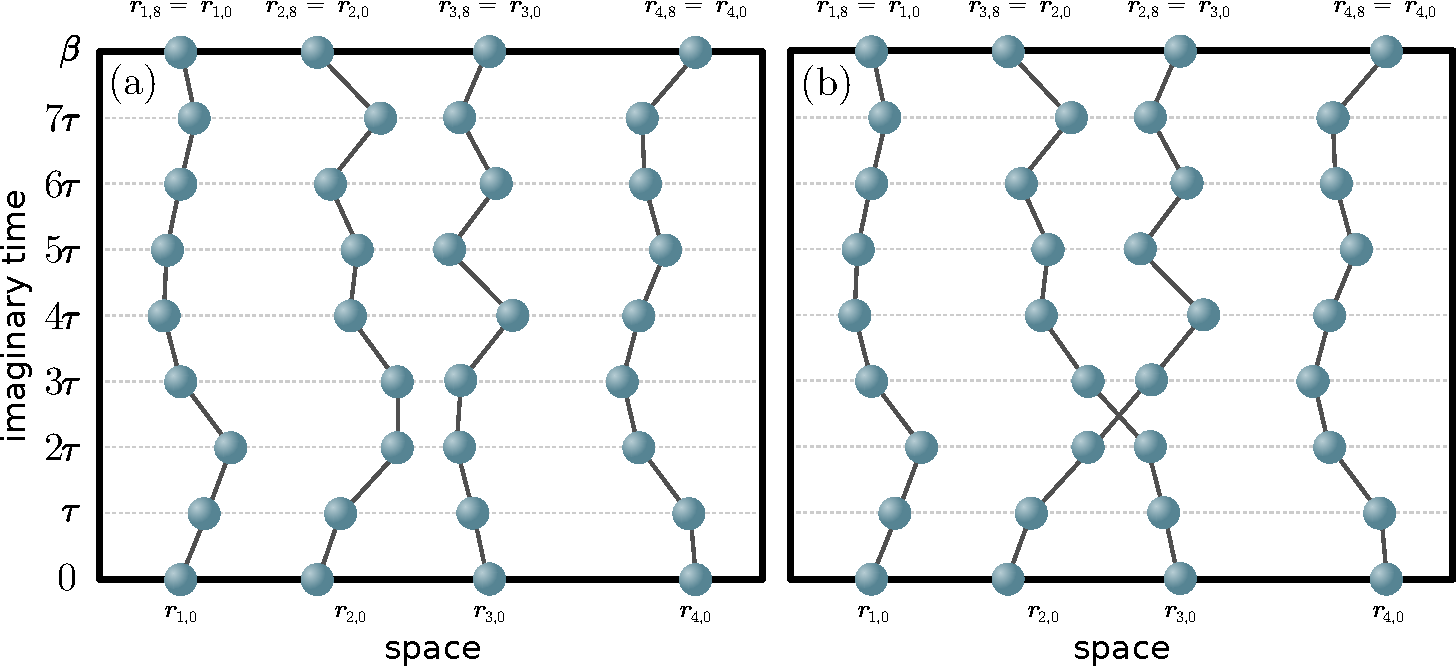
\includegraphics[width=0.75\columnwidth]{Figures/worldlines.pdf}
\end{center}
\caption{A sample configuration $N=4$ particles in $d$ spatial dimensions ($d=1$
here) where we have chosen $M=8$ such that $\tau = \beta/8$. The actual
spatial positions of the particles are identical in panels (a) and (b),
however they differ by a reconnection between imaginary times $2\tau$ and $3\tau$
corresponding to a permutation of the particle labels $|R_8\rangle_\mathrm{a} =
|R_0\rangle = |\vec{r}_{1,0},\vec{r}_{2,0},\vec{r}_{3,0},\vec{r}_{4,0}\rangle$
while $|R_8\rangle_\mathrm{b} =
\hat{\mathcal{P}}|R_0\rangle =
|\vec{r}_{1,0},\vec{r}_{3,0},\vec{r}_{2,0},\vec{r}_{4,0}\rangle$.}
\label{fig:config}
 \end{figure}
% ---------------------------------------------------------------------------------
%
These worldlines are composed of a series of ``beads'' which represent the
spatial positions of the particles at a given imaginary time slice and a set of
links which connect them and define a permutation of particle labels.  Thus,
the primary data structures used to store the configurations of the system
include a $d \times N \times M$ tensor for the positions and a $2 \times N
\times M$ tensor for the links allowing for the identification of any bead
$\vec{r}_{i,\alpha}$ and its imaginary time neighbor at $\vec{r}_{i,\alpha+1}$.

Motivated by the imaginary time boundary condition $|\R_M\rangle =
\hat{\mathcal{P}}|\R_0\rangle$, Chandler and Wolynes \cite{Chandler:1981gz}
introduced an alternative way to think about the worldlines in terms of an
isomorphism to classical ``ring polymers''.  Under the identity permutation,
these polymers consist of $M$ beads, but as permutations take place, the number
of beads can grow to some $n M$ where $1 \le n \le N$. This can be most easily
visualized in two spatial dimensions as shown in Figure~\ref{fig:polymers}.
%
% ---------------------------------------------------------------------------------
\begin{figure}
\begin{center}
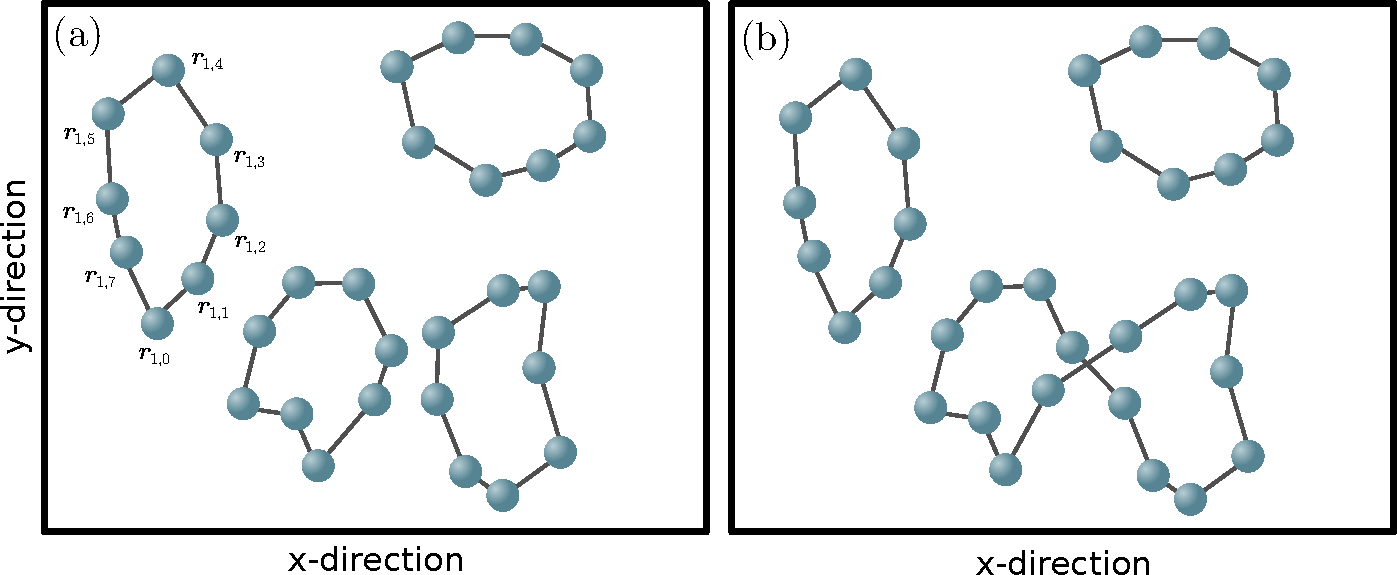
\includegraphics[width=0.75\columnwidth]{Figures/polymers.pdf}
\end{center}
\caption{Discrete particle worldlines can also be viewed as classical ring
    polymers where only beads on the same imaginary time slice interact between
    polymers.  Here we have again chosen $N=4$ and $M=8$ with (a) and (b)
    differing by a particle permutation, which in this picture results in the
``linking'' of spatially adjacent polymers.}
\label{fig:polymers}
 \end{figure}
% ---------------------------------------------------------------------------------
%
We can now make a number of important observations:
\begin{enumerate}
    \item A classical particle would consist of a ``polymer'' of zero radius.
    \item The spatial extent of a polymer is related to the thermal de Broglie
    wavelength $\lambda_{\mathrm{dB}} = \sqrt{2\pi \hbar^2 / m k_\mathrm{B} T
    }$.
\item For a finite size system with periodic boundary conditions, worldlines
    can \emph{wind} around the cell as the number of beads per polymer grows
    via permutations which are more favorable at low temperatures.  The width
    of the distribution of integer winding numbers is related to the superfluid
    fraction.
\end{enumerate}

\subsection{Weights}
%-------------------
Now that we have identified our configurations, in order to devise a sampling
scheme we must return to the partition function in \eqref{eq:Zpermute} and
attempt to compute the weights.  Our construction thus far has been
approximation free, and we have yet to utilize the fact that the new form of
the partition function includes the elements of effective high temperature
density matrices in the limit where $M \gg 1$. Consider a single transition
amplitude:
%
\begin{align}
\rho(\R_\alpha, \R_{\alpha+1}; \tau) &= \langle \R_\alpha | \e{-\tau(\hat{T} +
\hat{V})}|\R_{\alpha+1}\rangle
\end{align}
%
where we can now ignore the fact that $[\hat{\mathcal{T}},\hat{\mathcal{V}}]
\ne 0$ at the cost of an error that grows as $\tau^2$.  This is the
\emph{Primitive Approximation} and the error can be made arbitrarily small at a
given temperature at the linear cost of increasing $M$.  In practice, we can
utilize various schemes to drastically improve the error by explicitly
evaluating the commutator that appears in \eqref{eq:BCH} and we have chosen to 
employ a fourth order scheme called the generalized Suzuki factorization
\cite{Jang:2001cl}. For the purposes of these lecture notes, the primitive
approximation will be sufficient to illustrate all concepts and we can write
%
\begin{align}
    \rho(\R_\alpha, \R_{\alpha+1}; \tau) &= \langle \R_\alpha | 
    \e{-\tau\hat{\mathcal{T}}} \e{-\tau\hat{\mathcal{V}})}|R_{\alpha+1}\rangle + \mathrm{O}(\tau^2)
\nonumber \\
&= \int \mathcal{D}\R'\, \langle \R_\alpha | 
\e{-\tau\hat{\T}}|\R'\rangle \langle \R' | \e{-\tau\hat{\mathcal{V}})}|\R_{\alpha+1}\rangle 
\nonumber \\
&= \int \mathcal{D}\R'\, \langle \R_\alpha | 
\e{-\tau\hat{\T}}|\R'\rangle \langle \R' |\R_{\alpha+1}\rangle \e{-\tau
\mathcal{V}(\R_{\alpha+1})} \nonumber \\
&= \int \mathcal{D}\R'\, \langle \R_\alpha | 
\e{-\tau\hat{\T}}|\R'\rangle \delta (\R'-\R_{\alpha+1}) \e{-\tau
\mathcal{V}(\R_{\alpha+1})} \nonumber \\
&=  \langle \R_\alpha | \e{-\tau\hat{\T}}|\R_{\alpha+1}\rangle  \e{-\tau
\mathcal{V}(\R_{\alpha+1})} 
\label{eq:rhoPrimitive}
\end{align}
%
where we have inserted a complete set of states in line 2 and utilized the fact
that the potential energy operator is diagonal in imaginary time. We have
introduced a slight abuse of the set notation
$\R = \{\vec{r}_1, \cdots, \vec{r}_N \}$ where, for example, the Dirac delta
function is understood to mean
%
\begin{equation}
    \delta(\R-\R') \equiv \prod_{i=1}^{N}\delta(\vec{r}_i-\vec{r}'_i)
\end{equation}
%
and 
%
\begin{equation}
    \mathcal{V}(\R) \equiv \sum_{i=1}^N V(\vec{r}_i) + \frac{1}{2}\sum_{i,j}
U(\vec{r}_i-\vec{r}_j).
\end{equation}
%
Since the kinetic energy operator $\hat{\T}$ is clearly not diagonal in the
spatial position basis, in order to compute the first term in
\eqref{eq:rhoPrimitive} we can write the position eigenstate in terms of free
particle plane waves
%
\begin{align}
    |\R \rangle &=  | \vec{r}_1, \cdots, \vec{r}_N \rangle \nonumber \\
                &= \prod_{i=1}^N \int \frac{d\vec{k}_i}{(2\pi)^d} 
    \e{i \vec{k}_i \cdot \vec{r}_i} | \vec{k}_1, \cdots, \vec{k}_N\rangle.
\end{align}
%
Defining
%
\begin{equation}
    \lambda \equiv \frac{\hbar^2}{2 m}
\end{equation}
%
we can write
%
\begin{align}
    \langle \R | \e{-\tau\hat{\T}}|\R'\rangle &= \prod_{i=1}^N 
    \int \frac{d\vec{k}_i}{(2\pi)^d} \int \frac{d\vec{k}'_i}{(2\pi)^d} 
    \e{-i \vec{k}_i \cdot \vec{r}_i} \e{i \vec{k}'_i \cdot \vec{r}'_i} 
    \left \langle \vec{k}_1, \cdots, \vec{k}_N \left | \e{-\tau \lambda
\sum_{j=1}^N\hat{\vec{\nabla}}_j^2} \right | \vec{k}'_1, \cdots, \vec{k}'_N
\right \rangle \nonumber \\
&= \prod_{i=1}^N\int \frac{d\vec{k}_i}{(2\pi)^d} \int \frac{d\vec{k}'_i}{(2\pi)^d} 
\e{-\lambda \tau |\vec{k}'|^2 - i \vec{k}_i \cdot \vec{r}_i + i \vec{k}'_i \cdot
\vec{r}'_i} \left \langle \vec{k}_1, \cdots, \vec{k}_N | \vec{k}'_1, \cdots,
\vec{k}'_N \right \rangle \nonumber \\
&= \prod_{i=1}^N\int \frac{d\vec{k}_i}{(2\pi)^d} \int \frac{d\vec{k}'_i}{(2\pi)^d} 
\e{-\lambda \tau |\vec{k}'|^2 - i \vec{k}_i \cdot \vec{r}_i + i \vec{k}'_i \cdot
\vec{r}'_i}  (2\pi)^d \delta(\vec{k}_i-\vec{k}'_i) \nonumber \\
&= \prod_{i=1}^N\int \frac{d\vec{k}_i}{(2\pi)^d} 
\e{-\lambda \tau |\vec{k}|^2 + i \vec{k}_i \cdot (\vec{r}'_i - \vec{r}_i)}  
\nonumber \\
&= (4\pi \lambda \tau)^{-Nd/2} \mathrm{exp}\,\left( -\frac{1}{4\lambda
\tau} \sum_{i=1}^N | \vec{r}_i-\vec{r}'_i|^2 \right) 
\end{align}
%
which is just the free particle propagator that can be written in our set
notation as
%
\begin{align}
\rho_0(\R,\R';\tau) &=  \left \langle \R \left| \e{-\tau \hat{\T}} \right| \R' \right\rangle
    \nonumber \\
    &= (4\pi \lambda \tau)^{-Nd/2} \e{-\frac{1}{4\lambda \tau} | \R-\R'|^2}.
\label{eq:rho0}
\end{align}
%
We may now insert our complete expression for the primitive imaginary time
propagator
%
\begin{equation}
    \rho(\R_\alpha,\R_{\alpha+1};\tau) = \rho_0(\R_\alpha,\R_{\alpha+1};\tau)
\e{- \tau \mathcal{V}(\R_\alpha)}
\end{equation}
%
into the partition function in \eqref{eq:Zpermute} to find
%
\begin{align}
    \mathcal{Z}  &= (4\pi \lambda \tau)^{-NMd/2} 
    \frac{1}{N!}\sum_{\mathcal{P}} 
    \prod_{\alpha=0}^{M-1}\int \mathcal{D}\R_\alpha\,
\e{-\frac{1}{4\lambda \tau} | \R_\alpha-\R_{\alpha+1}|^2 - \tau
\mathcal{V}(\R_\alpha)} \nonumber \\
&= (4\pi \lambda \tau)^{-NMd/2}
    \frac{1}{N!}\sum_{\mathcal{P}} 
\prod_{\alpha=0}^{M-1}\prod_{i=1}^N 
\int d\vec{r}_{i,\alpha} \exp\left\{ 
    -\sum_{\alpha=0}^M\sum_{i=1}^N
    \left[\frac{|\vec{r}_{i,\alpha+1}-\vec{r}_{i,\alpha}|^2}{4\lambda \tau}  +
        \tau V(\vec{r}_{i,\alpha}) + \frac{\tau}{2}\sum_{j=1}^{N}
    U(\vec{r}_{i,\alpha}-\vec{r}_{j,\alpha})\right]
\right\}.
\label{eq:primitiveZ}
\end{align}
%
Because of the product of $M$ copies of the primitive propagator, the finite
Trotter error we make in the partition function is $\mathrm{O}(\tau)$. This
partition function is then just a ``path'' integral over all
possible configurations and permutations of particle worldlines where the
weight of each configuration is just the exponentiated effective action.

\subsection{Updates}
%-------------------
In order to sample configurations we must devise a series of updates that can
be proposed and accepted or rejected based on their weights.  We are aided by
the fact that it is possible to exactly sample the free density matrix
$\rho_0(\R,\R';\tau)$ since it is just a product of Gaussians.  This will allow
us to sample the kinetic part of the action in the ensemble and only consider
the potential action in the weights. We will outline two types of simple updates,
center-of-mass and staging moves, and briefly discuss a third permutation move
that will present us with a difficult challenge.


\subsubsection{Center of Mass}
%~~~~~~~~~~~~~~~~~~~~~~~~~~~~~
%
% ---------------------------------------------------------------------------------
\begin{figure}
\begin{center}
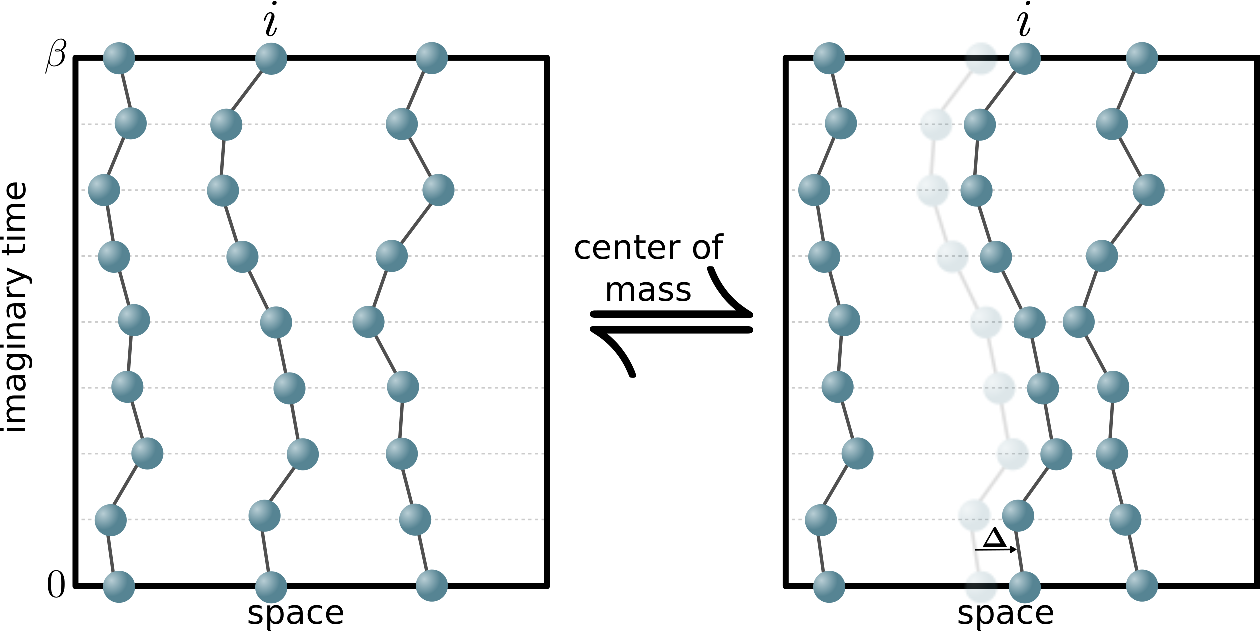
\includegraphics[width=0.70\columnwidth]{Figures/centerofmass.pdf}
\end{center}
\caption{A \emph{center of mass} Monte Carlo update, which translates the entire
worldline $i$ by a vector displacement $\vec{\Delta}$ without modifying the
connections between beads.}
\label{fig:com}
 \end{figure}
% ---------------------------------------------------------------------------------
%
A center-of-mass update involves the spatial translation of an entire
worldline, leaving the kinetic part of the action unchanged.  It is shown
schematically in Figure~\ref{fig:com} and proceeds as
follows:
\begin{enumerate}
    \item Choose a random integer $i \in [0,N-1]$ fixing worldline $i$ with beads located
        at $\vec{r}_{i,\alpha}$.
    \item Generate uniformly distributed random numbers, $\Delta_a$, where
        $a=1,\ldots,d$ on $(-\delta/2,\delta/2)$ where $\delta$ is a small number that can be
    modified to optimize the acceptance rate. Construct the vector $\vec{\Delta} =
    (\Delta_1,\ldots,\Delta_d)$.
\item Translate the entire worldline by $\vec{\Delta}$ to obtain a new set of
coordinates $\vec{r}'_{i,\alpha}$ where  $\vec{r}'_{i,\alpha} =
\vec{r}_{i,\alpha} + \vec{D}$ for $\alpha = 0,\ldots,M-1$.
\item Accept the update with probability
    %
\begin{equation}
    P_{\text{com}} = \mathrm{min} 
    \left\{1,\e{-\tau[\mathcal{V}(\vec{r}'_i)-\mathcal{V}(\vec{r}_i)]} \right\}
\end{equation}
%
where 
%
\begin{equation}
    \mathcal{V}(\vec{r_i}) \equiv \sum_{\alpha=0}^{M-1}\left[ V(\vec{r}_{i,\alpha}) + \frac{1}{2}\sum_{j=1}^{N}
    U(\vec{r}_{i,\alpha}-\vec{r}_{j,\alpha})\right].
\end{equation}
%
\end{enumerate}

\subsubsection{Staging}
%~~~~~~~~~~~~~~~~~~~~~~
%
% ---------------------------------------------------------------------------------
\begin{figure}
\begin{center}
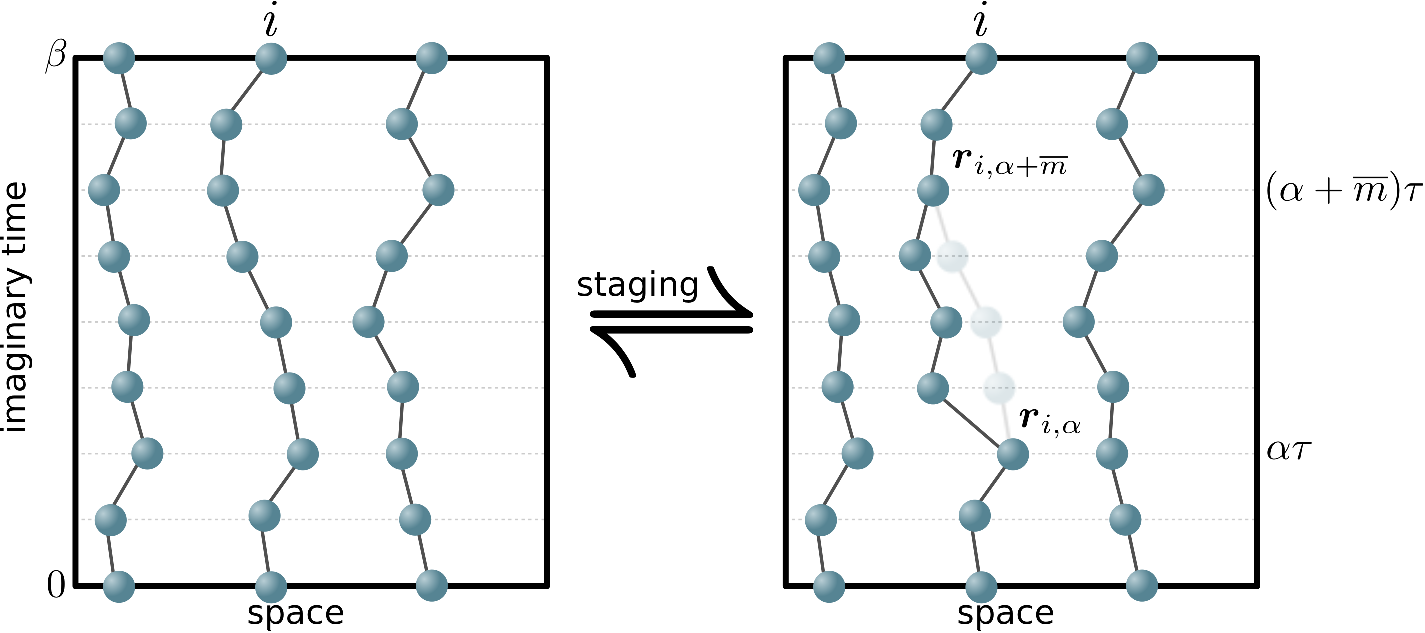
\includegraphics[width=0.75\columnwidth]{Figures/staging.pdf}
\end{center}
\caption{A \emph{staging} Monte Carlo update which uses the L\'{e}vy
construction to exactly sample the product of $\overline{m}$ free particle
density matrices connecting spatial positions $\vec{r}_{i,\alpha}$ and
$\vec{r}_{i,\alpha+\overline{m}}$.}
\label{fig:staging}
 \end{figure}
% ---------------------------------------------------------------------------------
%
A staging update \cite{Sprik:1985bz} generates a new section of path between
two fixed beads at time slices $\alpha$ and $\alpha+\overline{m}$ where
$\overline{m} < M$ is an algorithmic parameter that can be tuned to optimize
the acceptance rate. It
utilizes the fact that the free particle density matrix in \eqref{eq:rho0} is
Gaussian and thus obeys a convolution relation.  The problem is as follows:
given two known spatial positions (beads) on worldline $i$, say $r_{i,\alpha}$
and $r_{i,\alpha+\overline{m}}$, how do we exactly sample the product of free particle
density matrices:
%
\begin{equation}
    \rho_0(\vec{r}_{i,\alpha},\vec{r}_{i,\alpha+1};\tau) \cdots
    \rho_0(\vec{r}_{i,\alpha+\overline{m}-1},\vec{r}_{i,\alpha+\overline{m}};\tau)?
\end{equation}
%
The solution comes by choosing a single term in this product and constructing
the probability distribution for propagation to that position, constrained by the
endpoints. Let us drop the worldline index $i$ for brevity:  
%
\begin{align}
    \pi_0(\vec{r}_\gamma| \vec{r}_{\alpha},\vec{r}_{\alpha+\overline{m}}) &=
    \rho_0(\vec{r}_\alpha,\vec{r}_\gamma;(\gamma-\alpha)\tau) 
\rho_0(\vec{r}_\gamma,\vec{r}_{\alpha+\overline{m}};(\alpha+\overline{m}-\gamma)\tau) \nonumber \\
&\propto 
\exp\left[-\frac{|\vec{r}_\gamma-\vec{r}_{\alpha}|^2}{4\lambda (\gamma-\alpha)\tau} \right]
\exp\left[-\frac{|\vec{r}_{\alpha+\overline{m}}-\vec{r}_{\gamma}|^2}{4\lambda
(\alpha+\overline{m}-\gamma)\tau} \right]
\nonumber \\
&\propto \exp\left[-\frac{|\vec{r}_\gamma-\overline{\vec{r}}_{\gamma}|^2}{2 \sigma^2}\right]
\label{eq:pi0}
\end{align}
%
where 
%
\begin{align}
    \overline{\vec{r}}_\gamma &= \frac{1}{\overline{m}}
    \left[(\alpha+\overline{m}-\gamma)\vec{r}_{\alpha} +
    (\gamma-\alpha)\vec{r}_{\alpha+\overline{m}}\right] \nonumber \\
    \sigma^2 &= \frac{2\lambda}{\frac{1}{(\alpha + \overline{m}\gamma)\tau} +
\frac{1}{(\gamma-\alpha)\tau}}.
\end{align}
%
As \eqref{eq:pi0} is a simple Gaussian with mean $\overline{\vec{r}}_\gamma$ and
variance $\sigma^2$, it can be exactly sampled.  We are now ready to construct
our staging move, which is shown in Figure~\ref{fig:staging}:
\begin{enumerate}
    \item Choose a random integer $i \in [0,N-1]$ which fixes a worldline.
    \item Choose a random integer $\alpha \in [0,M-1]$ such that the start of
        the state occurs at $\vec{r}_{i,\alpha}$ and it ends at
        $\vec{r}_{i,\alpha+\overline{m}}$.  These beads are held fixed during
    the update.  \item Using $\vec{r}_{i,\alpha}$ and
        $\vec{r}_{i,\alpha+\overline{m}}$ construct the set of new positions
        $\{\vec{r}'_{i,\alpha+1},\ldots,\vec{r}'_{i,\alpha+\overline{m}-1}\}$ by exactly
        sampling \eqref{eq:pi0} for $\gamma = \alpha+1,\ldots,\alpha+m-1$.
    \item Accept the move with probability
    %
\begin{equation}
    P_{\text{com}} = \mathrm{min} 
    \left\{1,\e{-\tau[\mathcal{V}(\vec{r}'_i)-\mathcal{V}(\vec{r}_i)]} \right\}
\end{equation}
%
where 
%
\begin{equation}
    \mathcal{V}(\vec{r_i}) = \sum_{\gamma=\alpha}^{\alpha+m-1}\left[ V(\vec{r}_{i,\alpha}) + \frac{1}{2}\sum_{j=1}^{N}
    U(\vec{r}_{i,\gamma}-\vec{r}_{j,\gamma})\right].
\end{equation}
%
\end{enumerate}

\subsubsection{Permutation Sampling}
%~~~~~~~~~~~~~~~~~~~~~~~~~~~~~~~~~~~
We now address the point of how one can sample the sum over permutations of
particle labels in \eqref{eq:primitiveZ}. This is an onerous task, as for $N$
particles there are $N!$ possible permutations.  Historically this problem was
addressed in a brute force manner, by explicitly sampling all possible
reconnections of worldlines, however this limited the total number of
particles that could be efficiently simulated at low temperature to $N \sim
100$. In 2006, Boninsegni, Prokof'ev and Svistunov introduced a generalization
of a previous path integral based lattice quantum Monte Carlo scheme
\cite{Prokofev:1998ux} that has come to be known as the continuous space
\emph{worm} algorithm \cite{Boninsegni:2006ed,Boninsegni:2006gc}.


\section{Continuous Space Worm Algorithm}
%========================================

The worm algorithm \cite{Boninsegni:2006ed,Boninsegni:2006gc} (WA) solves the following two problems:
\begin{enumerate}
    \item Generalizes the configuration space to allow for simulations of
        interacting particles in the spatial continuum in the grand canonical
        ensemble.
    \item Solves the permutation problem by allowing for the sampling of
        topologically inequivalent winding sectors using only local updates.
\end{enumerate}
This is accomplished by extending the configuration space of worldlines
discussed in Section~\ref{sec:configurations} to include ``worms'' which are
open worldlines containing a \emph{head} at time slice $\alpha_h $ and \emph{tail} at
$\alpha_t$ with a variable imaginary time extent $(\alpha_h -
\alpha_t)\tau$.  The partition function governing the new system can be written
as
%
\begin{equation}
    \mathcal{Z}_W = \sum_{N=0}^{\infty} \mathcal{Z}(N) \e{\beta \mu N} + C
    \sum_{\alpha_h,\alpha_t} \int d\vec{r}_h \int d\vec{r}_t\,
    g\left(\vec{r}_h,\vec{r}_t; \alpha_h\tau-\alpha_t \tau\right)
\end{equation}
%
where $Z(N)$ is the canonical partition function at fixed particle number $N$
in \eqref{eq:Zpermute}, $\mu$ is the grand canonical chemical potential and
$g(\vec{r},\vec{r'};\tau-\tau')$ is (up to a normalization constant)
equal to the single particle Matsubara Green function
%
\begin{equation}
    g(\vec{r},\vec{r'};\tau-\tau') \equiv \mathcal{Z}(N)\left \langle 
\hat{\mathsf{T}}_\tau \hat{\psi}(\vec{r},\tau)\hat{\psi}^\dagger(\vec{r}',\tau')
\right \rangle
\end{equation}
%
with $\hat{\mathsf{T}}_\tau$ the imaginary time ordering operator. Working
in this extended ensemble requires us to extend the configuration space to
include open worldlines as shown in Figure~\ref{fig:worm}.  
%
% ---------------------------------------------------------------------------------
\begin{figure}
\begin{center}
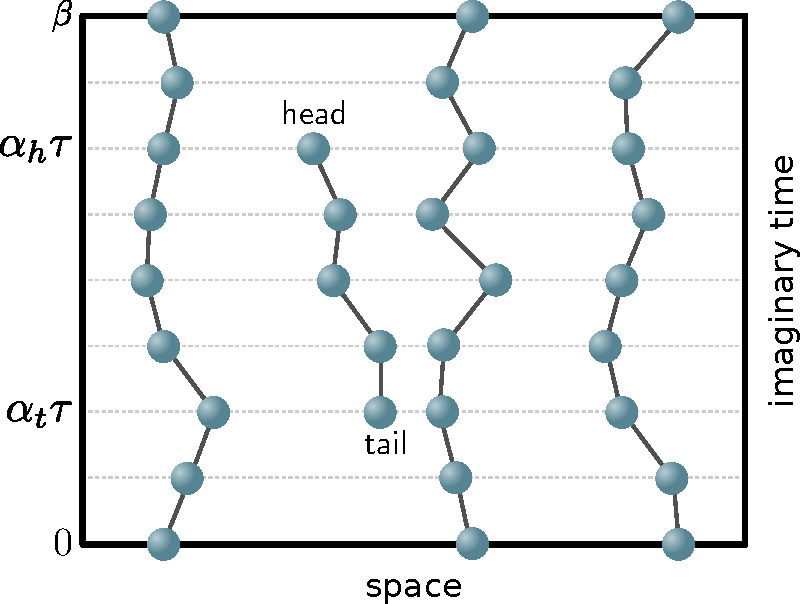
\includegraphics[width=0.40\columnwidth]{Figures/worm.pdf}
\end{center}
\caption{A sample configuration $N=3$ particles and one \emph{worm} in $d$
spatial dimensions ($d=1$ here) where we have chosen $M=8$ such that $\tau
= \beta/8$. The worm \emph{head} is located at imaginary time $\alpha_h \tau$ while
the \emph{tail} is at $\alpha_t \tau$. The imaginary time ``length'' of the worm is
equal to $(\alpha_h-\alpha_\tau)\tau = 4\tau$ here.}
\label{fig:worm}
 \end{figure}
% ---------------------------------------------------------------------------------
%
Such configurations are unphysical however, and we only make measurements of
observables when there are no worms present in the simulation. We refer to the
configurations of $\mathcal{Z}(N)$ as \emph{diagonal}, while those containing
worms are \emph{off-diagonal}. The numerical constant $C$ is of order one and
can be tuned to change the relative amount of Monte Carlo time spent in each
ensemble. 


\subsection{Worm Updates}
%-------------------
The worm updates come in complimentary pairs that satisfy detailed balance
together except for the \emph{swap} update, which provides the solution to the
permutation sampling problem described above. Much of the notation in this
section is taken directly from the original papers in
Refs.~[\onlinecite{Boninsegni:2006ed}] and [\onlinecite{Boninsegni:2006gc}].
In the following descriptions, when moving along worldlines, all addition of
time slices is understood to be performed modulo $M$ subject to the constraint
that $\{\vec{r}_{1,0},\ldots,\vec{r}_{N,0}\} = 
\{\vec{r}_{{\mathcal{P}}(1),M},\ldots,\vec{r}_{{\mathcal{P}}(N),0}\}$.

\subsubsection{Open/Close}
%~~~~~~~~~~~~~~~~~~~~~~~~~
An \emph{open} update, depicted in Figure~\ref{fig:openclose}, moves the
ensemble from diagonal to off-diagonal, and can only be attempted when there
are no worms present.  
%
% ---------------------------------------------------------------------------------
\begin{figure}
\begin{center}
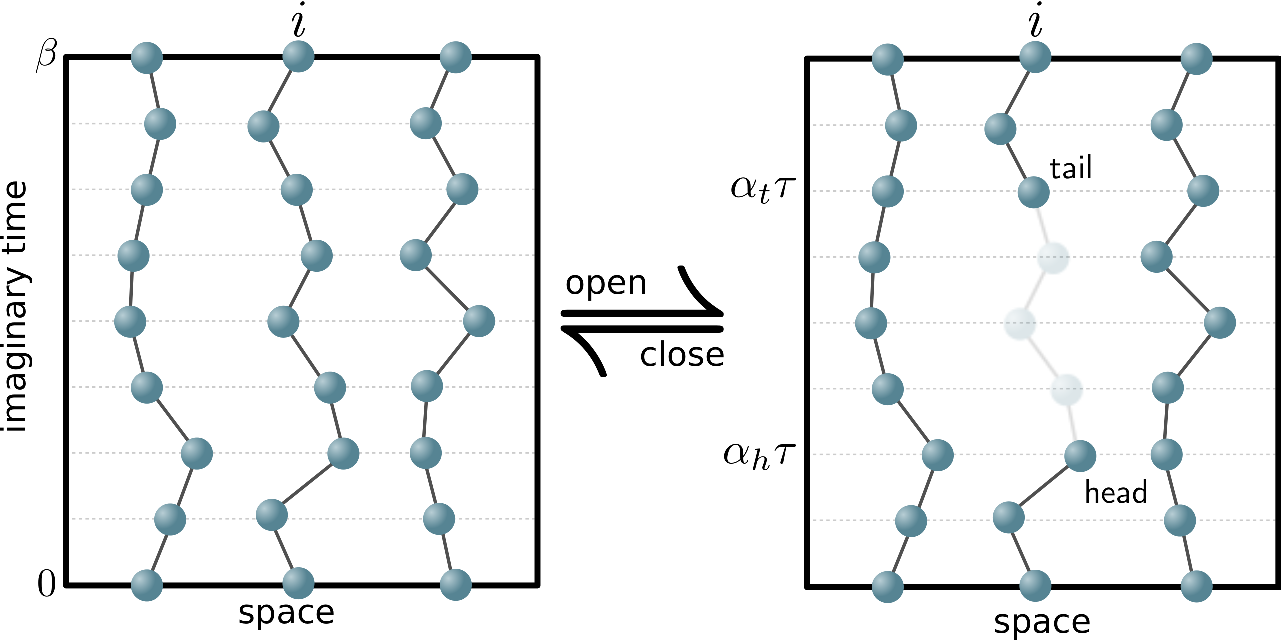
\includegraphics[width=0.70\columnwidth]{Figures/openclose.pdf}
\end{center}
\caption{The \emph{open} and \emph{close} complimentary Monte Carlo updates.
For an open move, we select a worldline $i$ and an imaginary time slice
$\alpha_h$.  $\overline{m}$ beads are then removed from the configuration,
moving to the off-diagonal ensemble and reducing the total number of physical
particles by one.  The close move operates in the reverse fashion, where a new
portion of worldline is constructed between the head and the tail of a worm,
resulting in a diagonal configuration with an additional particle.}
\label{fig:openclose}
 \end{figure}
% ---------------------------------------------------------------------------------
%
It proceeds as follows:

\begin{enumerate}
    \item Choose a random integer $i \in [0,N-1]$ fixing worldline $i$ with beads located
        at $\vec{r}_{i,\alpha}$.
    \item Generate a random integer $\alpha_h \in [0,M-1]$; this
        will be the location of the head of the proposed worm.
    \item Generate a random integer $m \in [0,\overline{m}-1]$ where $\overline{m} <
        M$ is a parameter to be optimized. Starting at time slice $\alpha_h$,
        find $\alpha_t = \alpha_h + m$, which will be the time slice of the tail.
    \item Remove the set of $m-1$ beads
        $\{\vec{r}_{i,\alpha_h+1},\ldots,
    \vec{r}_{,\alpha_h+m-1}\}$ where the addition is
    understood to be modulo $M$ subject to the imaginary time boundary
    condition $\vec{r}_{i,M} = \vec{r}_{\mathcal{P}(i),0}$ for a given
    permutation of particle labels.
\item Accept the move with probability
    %
\begin{equation}
P_{\text{open}} = \mathrm{min}\left[1, 
    \frac{C \overline{m} M N}{\rho_0(\vec{r}_{i,\alpha_h},\vec{r}_{i,\alpha_t};m\tau)}
\e{-\tau \Delta \mathcal{V} - \mu m \tau} \right]
\end{equation}
%
where $\Delta \mathcal{V}$ indicates the change in the total potential action,
which in this case is
%
\begin{equation}
    \Delta\mathcal{V} = -\sum_{\alpha=\alpha_h+1}^{\alpha_h+m-1} \left[ 
        V(\vec{r}_{i,\alpha}) + \frac{1}{2}\sum_{j=1}^N
        U(\vec{r}_{i,\alpha}-\vec{r}_{j,\alpha}) \right]
\end{equation}
%
and $\rho_0$ is the free particle propagator in \eqref{eq:rho0}.
\end{enumerate}
If the move is accepted, the configuration now contains $N \to N-1$ physical
particles and 1 worm.\\[2ex]

\noindent
The \emph{close} move, shown in Figure~\ref{fig:openclose}, provides a detailed balance compliment to \emph{open} and
moves the ensemble from off-diagonal back to diagonal. It is only possible when
a worm and $N$ particles are present and contains the following steps:
\begin{enumerate}
    \item Identify the ``particle'' label $i$ of the worm and the integer number of time steps, $m$ between $\alpha_h$ and
        $\alpha_\tau$ between the head and tail where we assume $\alpha_h > \alpha_t$ modulo $M$.
\item If $m=0$ or $m\ge \overline{m}$ reject the move immediately.
\item Otherwise, generate a new partial worldline containing $m-1$ particle positions connecting 
    $\vec{r}_{i,\alpha_h}$ and $\vec{r}_{i,\alpha_t}$: $\{\vec{r}'_{i,\alpha_h+1},\ldots,
    \vec{r}'_{,\alpha_h+m-1}\}$ where the individual positions are sampled from
    the product of $m$ free particle propagators
    $\prod_{\alpha=\alpha_h}^{\alpha_h+m-1}
    \rho_0(\vec{r}_{i,\alpha},\vec{r}_{i,\alpha+1};\tau)$.
\item Accept the move with probability
    %
\begin{equation}
    P_{\text{close}} = \mathrm{min} \left[1,
        \frac{\rho_0(\vec{r}_{i,\alpha_h},\vec{r}_{i,\alpha_t}; m \tau)}{C
    \overline{m}M (N+1)} \e{-\tau \Delta \mathcal{V} + \mu m \tau} \right]
\end{equation}
%
where
%
\begin{equation}
    \Delta\mathcal{V} = \sum_{\alpha=\alpha_h+1}^{\alpha_h+m-1} \left[ 
        V(\vec{r}'_{i,\alpha}) + \frac{1}{2}\sum_{j=1}^N
        U(\vec{r}'_{i,\alpha}-\vec{r}_{j,\alpha}) \right].
\end{equation}
%
\end{enumerate}
If the move is accepted, we are now in a configuration with $N \to N+1$
particles and no worms.

\subsubsection{Insert/Remove}
%~~~~~~~~~~~~~~~~~~~~~~~~~~~~
 An \emph{insert} move (Figure~\ref{fig:insertremove}) involves the addition to
 the ensemble of an entire worm and moves the configuration from diagonal to
 off-diagonal.  It is only possible if there are no worms present in the system
 and proceeds as follows:
\begin{enumerate}
    \item Choose a random integer $\alpha_t \in [0,M-1]$; this will be the
        location of the worm tail.
    \item Choose a random integer $m \in [0,\overline{m}-1]$, this will be the
        length of the worm.
    \item Randomly choose a position inside the simulation cell of volume $V$
        and label it $\vec{r}'_{i,\alpha_t}$ where $i$ is the particle label of
        the proposed worm.
    \item Generate a new partial worldline containing $m-1$ particle positions
        starting at position $\vec{r}'_{i,\alpha_t}$: $\{\vec{r}'_{i,\alpha_t+1},\ldots,
    \vec{r}'_{,\alpha_t+m}\}$ where the individual positions are sampled from
    the product of $m$ free particle propagators
    $\prod_{\alpha=\alpha_t}^{\alpha_t+m-1}
    \rho_0(\vec{r}_{i,\alpha},\vec{r}_{i,\alpha+1};\tau)$.
\item Accept the move with probability
    %
\begin{equation}
    P_{\text{insert}} = \mathrm{min} \left[1,
C V \overline{m}M \e{-\tau \Delta \mathcal{V} + \mu m \tau} \right]
\end{equation}
%
where
%
\begin{equation}
    \Delta\mathcal{V} = \sum_{\alpha=\alpha_t}^{\alpha_t+m} \left[ 
        V(\vec{r}'_{i,\alpha}) + \frac{1}{2}\sum_{j=1}^N
        U(\vec{r}'_{i,\alpha}-\vec{r}_{j,\alpha}) \right].
\end{equation}
%
\end{enumerate}
If the move is accepted, the simulation cell will contain $N$ particles and 1
worm.\\[2ex]
%
% ---------------------------------------------------------------------------------
\begin{figure}
\begin{center}
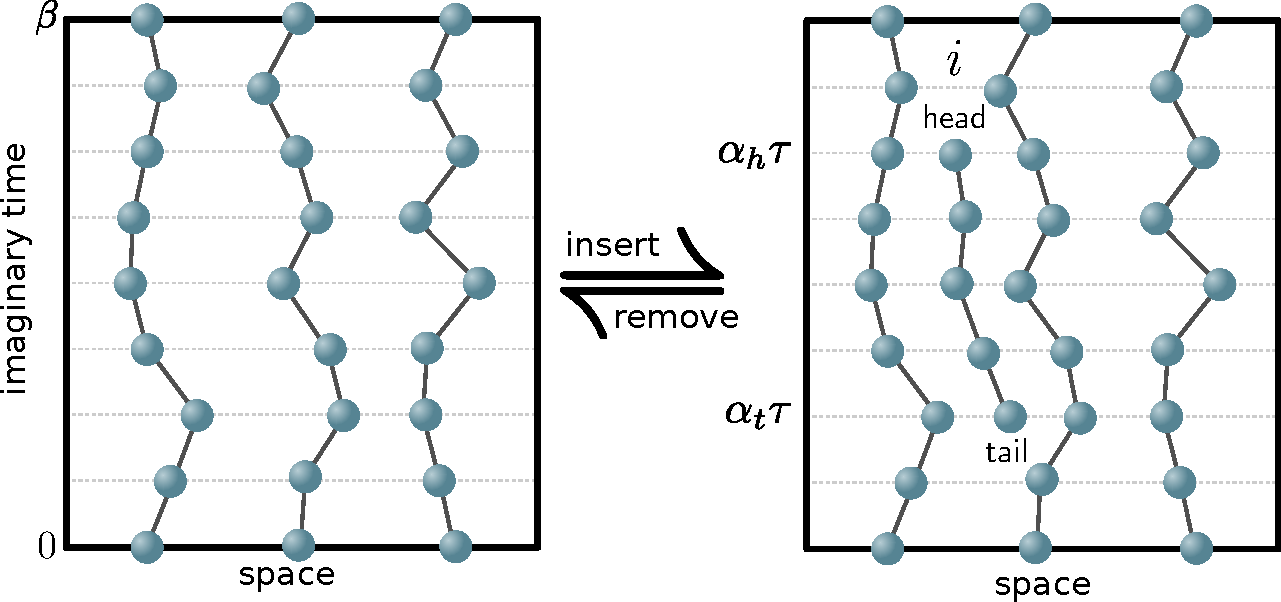
\includegraphics[width=0.70\columnwidth]{Figures/insertremove.pdf}
\end{center}
\caption{The \emph{insert} and \emph{remove} pair of Monte Carlo updates.  For
an insert move, a worm of imaginary time extent $m\tau = (\alpha_h -
\alpha_t)\tau$ is placed at a random set of positions in the simulation cell,
moving the configuration space to the off-diagonal ensemble.  The remove update
deletes all beads on worm, moving the simulation to the diagonal ensemble.} 
\label{fig:insertremove}
 \end{figure}
% ---------------------------------------------------------------------------------
%

\noindent
The \emph{remove} update deletes a worm from the configuration, moving the
ensemble from off-diagonal to diagonal. It is only possible if there is a worm
present and is undertaken as follows:
\begin{enumerate}
    \item Find the particle label of the worm, call it $i$, and the positions
        of the head and tail: $\vec{r}_{i,\alpha_h}$ and
        $\vec{r}_{i,\alpha_h}$.
    \item Determine $m = \alpha_h - \alpha_t$, the length of the worm.
    \item If $m > \overline{m}$ reject the move.
    \item Otherwise, delete the set of $m$ beads $\{\vec{r}_{i,\alpha_t},\ldots,
    \vec{r}'_{,\alpha_t+m}\}$.
\item Accept the move with probability
    %
\begin{equation}
    P_{\text{remove}} = \mathrm{min} \left[1,
    \frac{1}{C V \overline{m}M} \e{-\tau \Delta \mathcal{V} - \mu m \tau} \right]
\end{equation}
%
where
%
\begin{equation}
    \Delta\mathcal{V} = -\sum_{\alpha=\alpha_t}^{\alpha_t+m} \left[ 
        V(\vec{r}_{i,\alpha}) + \frac{1}{2}\sum_{j=1}^N
        U(\vec{r}_{i,\alpha}-\vec{r}_{j,\alpha}) \right].
\end{equation}
%
\end{enumerate}
If the move is accepted, the simulation cell will contain $N$ particles and 0
worms.

\subsubsection{Advance/Recede}
%~~~~~~~~~~~~~~~~~~~~~~~~~~~~~
The \emph{advance} and \emph{recede} updates, shown in
 Figure~\ref{fig:advancerecede} do not change the nature of the
ensemble and operate only in the off-diagonal case in the presence of a worm.
For advance:
\begin{enumerate}
    \item Determine the time slice $\alpha_h$ and spatial location
        $\vec{r}_{i,\alpha_h}$ of the worm head.
    \item Choose a random integer $m \in [0,\overline{m}-1]$.
    \item Generate a partial worldline composed of the set of new particle positions 
        $\{\vec{r}'_{i,\alpha_h+1},\ldots, \vec{r}'_{i,\alpha_h+m}\}$ which are
        sampled from $\prod_{\alpha=\alpha_h}^{\alpha_h+m-1}
    \rho_0(\vec{r}_{i,\alpha},\vec{r}_{i,\alpha+1};\tau)$.
\item Accept the move with probability
    %
\begin{equation}
    P_{\text{advance}} = \mathrm{min} \left[1,
    \e{-\tau \Delta \mathcal{V} + \mu m \tau} \right]
\end{equation}
%
where
%
\begin{equation}
    \Delta\mathcal{V} = \sum_{\alpha=\alpha_t+1}^{\alpha_t+m} \left[ 
        V(\vec{r}'_{i,\alpha}) + \frac{1}{2}\sum_{j=1}^N
        U(\vec{r}'_{i,\alpha}-\vec{r}_{j,\alpha}) \right].
\end{equation}
%
\end{enumerate}

%
% ---------------------------------------------------------------------------------
\begin{figure}
\begin{center}
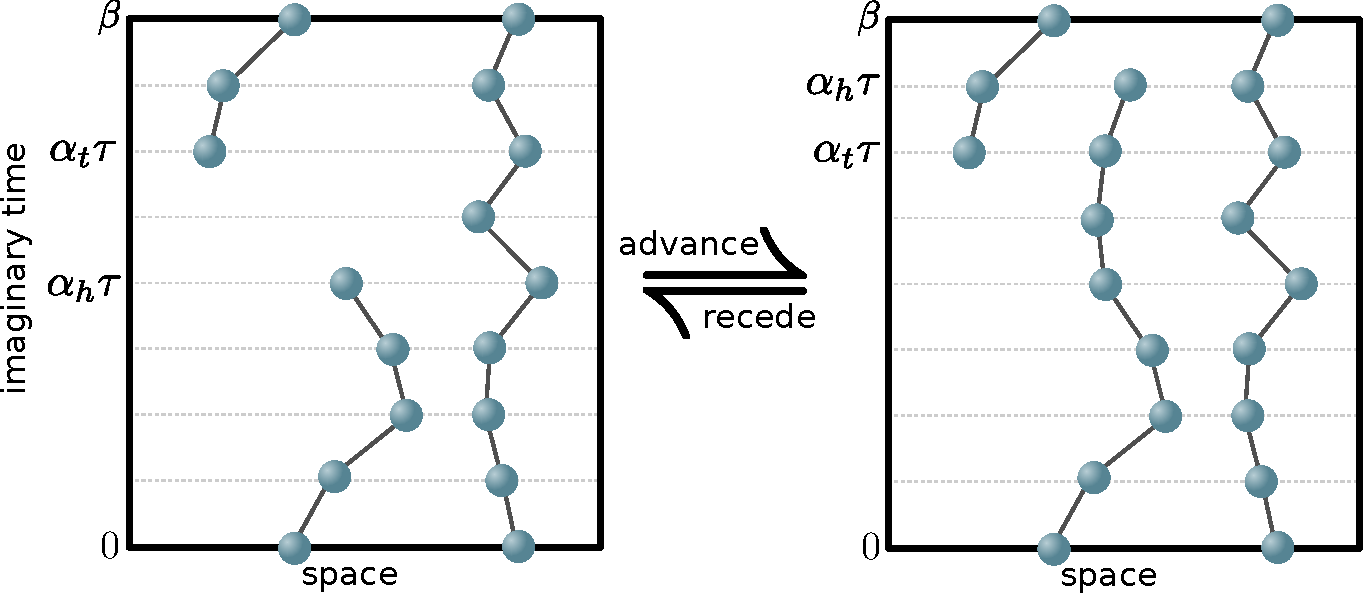
\includegraphics[width=0.70\columnwidth]{Figures/advancerecede.pdf}
\end{center}
\caption{The \emph{advance} and \emph{recede} Monte Carlo updates.  The advance
    move propagates the head of the worm forwards in imaginary time by
    generating a set of new spatial positions.  The recede move does the
opposite, deleting beads and reducing the length of the worm.}
\label{fig:advancerecede}
 \end{figure}
% ---------------------------------------------------------------------------------
%

\noindent
For recede:
\begin{enumerate}
    \item Determine the time slice $\alpha_h$ and spatial location
        $\vec{r}_{i,\alpha_h}$ of the worm head.
    \item Choose a random integer $m \in [0,\overline{m}-1]$.
    \item Delete the partial worldline containing the set of particle coordinates: 
        $\{\vec{r}_{i,\alpha_h-(m-1)},\ldots, \vec{r}_{i,\alpha_h}\}$.
\item Accept the move with probability
    %
\begin{equation}
    P_{\text{recede}} = \mathrm{min} \left[1,
    \e{-\tau \Delta \mathcal{V} - \mu m \tau} \right]
\end{equation}
%
where
%
\begin{equation}
    \Delta\mathcal{V} = -\sum_{\alpha=\alpha_h-(m-1)}^{\alpha_h} \left[ 
        V(\vec{r}'_{i,\alpha}) + \frac{1}{2}\sum_{j=1}^N
        U(\vec{r}'_{i,\alpha}-\vec{r}_{j,\alpha}) \right].
\end{equation}
%
\end{enumerate}
We note that similar copies of these updates could also be performed at the
tail of the worm, but such moves should be unnecessary for ergodicity in the presence of
imaginary time translation symmetry.

\subsubsection{Swap}
%~~~~~~~~~~~~~~~~~~~
The \emph{swap} update, shown in Figure~\ref{fig:swap} is behind the huge
speedup inherent in the worm algorithm, as it allows us to sample different
topological winding sectors (permutations) using only local updates.  It does
not, therefore, suffer from the horrendous $N!$ scaling of brute-force
permutation sampling. It only operates on off-diagonal configurations, in the
presence of a worm, and does not change the ensemble. It provides a method by
which a single worm grows by $n M$ time slices where $1 \le n \le N$ by
``swapping'' its head with a proximate unbroken particle worldline.  To
perform a swap move:
%
% ---------------------------------------------------------------------------------
\begin{figure}
\begin{center}
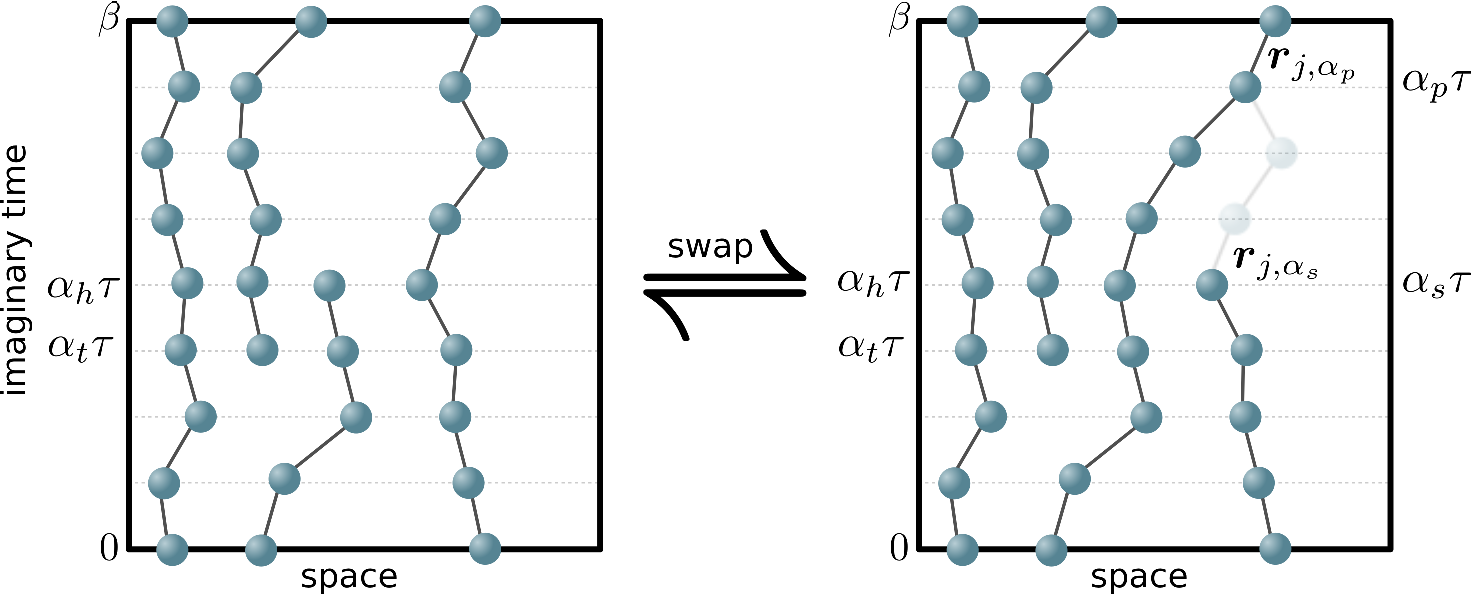
\includegraphics[width=0.70\columnwidth]{Figures/swap.pdf}
\end{center}
\caption{The \emph{swap} Monte Carlo update, which does not change the nature
of the ensemble, but allows for the sampling of different topological sectors.
A new partial worldline is generated between the head of the worm and a
neighboring particle worldline position at an advanced time slice.  The
original portion of the particle worldline is then erased, ``swapping'' the
head of the worm and increasing the imaginary time extent of the worm.}
\label{fig:swap}
 \end{figure}
% ---------------------------------------------------------------------------------
%
\begin{enumerate}
    \item Determine the time slice $\alpha_h$ and spatial location
        $\vec{r}_{i,\alpha_h}$ of the worm head.
    \item Advance to the time slice of the \emph{pivot} bead $\alpha_p =
        \alpha_h + \overline{m}$ where the addition is modulo $M$ and find the
        set of all beads $\ell_p \equiv \{\vec{r}_{k,\alpha_p}\}$ such that
        $|\vec{r}_{i,\alpha_h} - \vec{r}_{k,\alpha_p}| < R$ where $R \in
        \mathbbm{R}$ is a simulation parameter to be optimized.
\item Use tower sampling to select a single bead $\vec{r}_{j,\alpha_p} \in
    \{\vec{r}_{k,\alpha_p}\}$ from the list with probability
    %
\begin{equation}
    P_p = \frac{1}{\Sigma_p}
    \rho_0(\vec{r}_{i,\alpha_h},\vec{r}_{j,\alpha_p};\overline{m}\tau)
\end{equation}
%
where the normalization factor is
%
\begin{equation}
\Sigma_p = \sum_{\vec{r}\in\ell_p} 
    \rho_0(\vec{r}_{i,\alpha_h},\vec{r};\overline{m}\tau).
\end{equation}
%
\item Recede $\overline{m}$ time steps along worldline $j$ from $\alpha_p$ to
    identify the \emph{swap} bead at $\alpha_s = \alpha_h =
    \alpha_p-\overline{m}$: $\vec{r}_{j,\alpha_s}$. If the tail of the worm,
    $\vec{r}_{i,\alpha_t}$, is encountered during this process, immediately reject the move.
\item If $|\vec{r}_{j,\alpha_p} - \vec{r}_{j,\alpha_s}| \ge R$ reject the move.
\item Otherwise, create a second list $\ell_s \equiv \{\vec{r}_{k,\alpha_s}\}$ such
    that $|\vec{r}_{j,\alpha_s} - \vec{r}_{k,\alpha_p}| < R$ and form the sum
    %
\begin{equation}
\Sigma_s = \sum_{\vec{r}\in\ell_s} 
    \rho_0(\vec{r}_{j,\alpha_p},\vec{r};\overline{m}\tau).
\end{equation}
%
\item Delete the set of $\overline{m}-1$ beads
    $\{\vec{r}_{j,\alpha_s+1},\ldots,\vec{r}_{j,\alpha_s+m-1} \}$.
\item Construct a new partial worldline containing the set of particle
    positions $\{\vec{r}'_{i,\alpha_h+1},\ldots \vec{r}'_{i,\alpha_h+m-1}\}$
    connecting $\vec{r}_{i,\alpha_h}$ and $\vec{r}_{j,\alpha_p}$ sampled from
    the product of $\overline{m}$ free particle propagators
    $\prod_{\alpha=\alpha_h}^{\alpha_h+m-1}
    \rho_0(\vec{r}_{i,\alpha},\vec{r}_{i,\alpha+1};\tau)$ where
    $\vec{r}_{i,\alpha_h + m} = \vec{r}_{j,\alpha_p}$.
\item The head of the worm is now located at $\vec{r}_{j,\alpha_s}$ and its
    length has increased by the number of time slices contained in the 
    particle that was labeled by $j$.
\item Accept the move with probability
    %
\begin{equation}
    P_{\text{swap}} = \mathrm{min}\left[1,
        \frac{\Sigma_p}{\Sigma_s} \e{-\tau\Delta{\mathcal{V}}}
    \right]
\end{equation}
%
where 
\begin{equation}
    \Delta\mathcal{V} = \sum_{\alpha=\alpha_h}^{\alpha_h+\overline{m}} \left\{ 
        V(\vec{r}'_{i,\alpha}) - V(\vec{r}_{j,\alpha}) + \frac{1}{2}\sum_{k=1}^N
        \left[ U(\vec{r}'_{i,\alpha}-\vec{r}_{k,\alpha}) -
    U(\vec{r}_{j,\alpha}-\vec{r}_{k,\alpha})\right] \right\}.
\end{equation}
%
\end{enumerate}

\bibliographystyle{apsrev4-1}
\bibliography{refs}

\end{document}
